\chapter{Day 1 - Best Practices}
\paragraph{}This Code Summer School will cover the basics of Python and C++ as well as some best practices and good habits to develop early as programmers.  Whether you intend to pursue programming professionally or merely keep it as a skill in your back pocket, these lessons will hopefully serve as a good foundation.  I anticipate each day will be a couple of hours of lecture and practice, with Q\&A mixed in as we go.  I plan to keep it fairly informal, so questions and interruptions are fine and welcome.  Also, feedback is much appreciated as it will help to refine this Summer School for following years.

\begin{center}\rule{0.5\linewidth}{0.5pt}\end{center}

``Programming'' is such a hugely expansive term,
covering a staggering number of techniques, languages, processes,
hardware configurations, purposes, applications, scales, and so forth.

\emph{So what is programming, really?}

The short version is that programming is a way of making a computer
(another broad term!) perform tasks. These tasks can be as simple as the
addition of two numbers, or as complex as calculating the excited state
energy of a fluorescent nucleotide as it moves through a solution of
water and sodium chloride ions. As the tasks become more complex, the
code becomes more complex as well. Small tasks may be manageable with
tiny scripts or single-file programs, while larger ones may require the
inclusion of other tools, multiple files, and more complicated design
principles.

For the purposes of this Summer School, we'll mostly be sticking to the
introductory/entry-level stuff, but remember that the actual limits of
your programs are only in the capacity of your hardware and the breadth
of your imagination.

There are some rules to programming that should really be learned early
on, if only because knowing them early will make the rest considerably
easier. For many experienced programmers, the actual writing of code is
a smaller portion of the overall process than one might expect.

\textbf{Version Control} - This is a very important habit to get into.
In the simplest form, version control provides a means of keeping track
of the changes you've made to your code as you go, as well as providing
information about who made which changes in a collaborative project.
More complicated version control can lead to things like software
written for different types of hardware, or for different scales of
calculations, etc.

\textbf{Code Formatting} - Many different groups and companies have what
are known as ``style guides'' for any code produced in, by, or for the
organization. These often include the simple concepts like ``how many
spaces constitute a \texttt{tab} in your code?'' or ``What information,
if any, should be included in comments at the top of each file?''.
However, these style guides can also include more complex information
beyond text formatting and up into things like ``Each function
definition should include comments describing the arguments to the
function and what the function returns on completion'' or ``Test suites
must be included for all additions to the codebase before they may be
considered for merging''.

\textbf{Debugging} - This is a team effort, because invariably the
person who wrote the code might wind up missing some of their own
mistakes that others will readily find. This is not at all an indicator
of skill, intelligence, or character. This is purely because we can get
tunnel vision about our own code (it happens to the best of us), and
because our brains are wired to recognize \emph{and complete} patterns.
Where we might ``see'' a missing semicolon at the end of a line of code
we wrote because we expect it to be there, someone else who didn't write
our code may notice it immediately. Interestingly, debugging is actually
a \emph{highly} valued skill in industry, because fixing problems is
usually far more expensive than preventing them in the first place.

\textbf{Pseudocode} - Other names for pseudocode include ``algorithm
development'', ``project management'', ``outlining'', ``planning'',
``thinking'', and ``jotting that down so I don't forget it later''.
Pseudocoding is effectively writing out the stages of your program in
plain language (\emph{not code}) to ensure a clear understanding of the
problem you're trying to solve. Often, programmers will begin pseudocode
with a very simple set of steps they think of the problem. Each step can
be explained in more and more detail as a set of smaller, more
manageable steps, until eventually you wind up with a complete list of
steps that can be converted to computer commands. Pseudocode can also
provide some insight into ways the code might be optimized, such as by
revealing opportunities to parallelise the execution, or by revealing
regions where something being calculated can just be saved for reuse
rather than recalculated again later.

\textbf{Variable Types} - Different types of information can be stored
for use by the computer. Some programming languages are fairly lenient
about variable types and are flexible with what types of data are being
provided in a given variable. Others are a bit more strict, and require
explicit type declarations/definitions for each variable to ensure
proper memory allocation. \emph{If only some of that made sense, you're
in the right place.}

%%%%%%%%%%%%%%%%%%%%%%%%%%%%%%%%%%%%%%%%%%%%%%%%%%%%%%%%%%%%%%%%%%%%%%%%%%%%%%%%%%%%%%%%%%%%%%%%%%%%%%%%%%%%%%%%%%%%%
\section{Version Control, Git, and GitHub}
The most commonly used tool for version control is \texttt{git}, with
related websites \href{https://www.github.com}{GitHub},
\href{https://about.gitlab.com/}{GitLab}, and
\href{https://bitbucket.org/}{Bitbucket}. For the purposes of this
workshop, we'll focus on using GitHub because it's free and most (if not
all) of us already have accounts there.

There are a few steps to do first if you've never used \texttt{git} on
your current computer before. These will configure your computer for use
with your GitHub account. If you use multiple computers (including
working from a HPC/Supercomputer), these steps will need to be
configured for each computer you use.

\begin{center}\rule{0.5\linewidth}{0.5pt}\end{center}

Configure your local machine with an SSH-key. This will allow your
computer to connect to other \textbf{trusted} computers that you've
previously designated as such, and this includes your Github account.

\begin{Shaded}
\begin{Highlighting}[]
    \BuiltInTok{cd} \VariableTok{\$HOME}
    \FunctionTok{ssh{-}keygen}
\end{Highlighting}
\end{Shaded}

will give the following response/prompt:

\begin{verbatim}
    Generating public/private rsa key pair
    Enter file in which to save the key (/home/username/.ssh/id_rsa): 
\end{verbatim}

If the file already exists, choose a new filename such as
\texttt{git\_rsa} or something you'll recognize.

\begin{verbatim}
    Enter passphrase (empty for no passphrase): 
    Enter same passphrase again: 
\end{verbatim}

You can set a passphrase if you want, but keep in mind you'll be
entering it every single time you upload changes of your code to GitHub.
Some people choose not to have a passphrase for this particular aspect
of their work, others do.

\begin{verbatim}
    Your identification has been saved in /home/username/.ssh/git_rsa
    Your public key has been saved in /home/username/.ssh/git_rsa.pub
    The key fingerprint is:
    SHA256:8U9t+r+SwCi8Xe8uu3HCjbHa7WU51A9pArzm9+F+esk username@Computer
    The key's randomart image is:
    +---[RSA 3072]----+
    |                 |
    |       .         |
    |        +  . +   |
    |         =. =. ..|
    |      . S =*o.=..|
    |       = .oBo+..o|
    |        ..o+*o.*.|
    |       . o.+o*D .|
    |           +@Bo*o|
    +----[SHA256]-----+
\end{verbatim}
\begin{center}\rule{0.5\linewidth}{0.5pt}\end{center}
Add the SSH key to your GitHub Account to allow your computer to access
it.

Go to your account settings page and click on
\texttt{SSH\ and\ GPG\ keys}, then click on \texttt{New\ SSH\ key}.

\begin{figure}
\centering

\includegraphics[width=0.8\textwidth]{Images/GH_01.png}
\caption{GitHub Step 1}
\end{figure}
\FloatBarrier

\begin{figure}
\centering

\includegraphics[width=0.8\textwidth]{Images/GH_02.png}
\caption{GitHub Step 2}
\end{figure}
\FloatBarrier

\begin{figure}
\centering
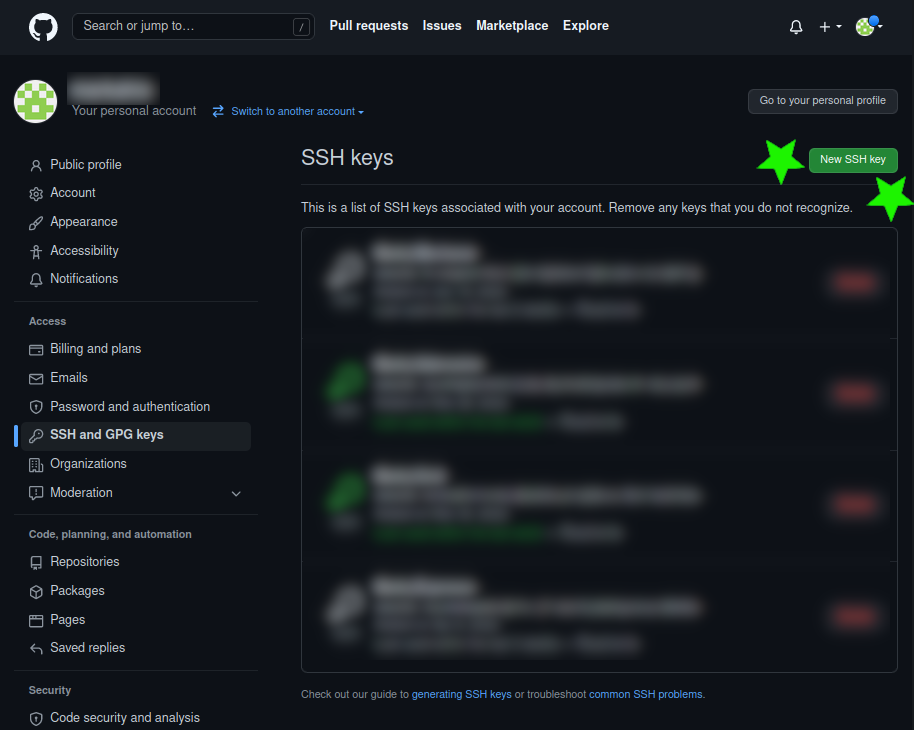
\includegraphics[width=0.8\textwidth]{Images/GH_03.png}
\caption{GitHub Step 3}
\end{figure}
\FloatBarrier

You'll need some text out of a file generated by the \texttt{ssh-keygen}
step. If you named the keyfile \texttt{git\_rsa}, the process will have
also produced a file called \texttt{git\_rsa.pub}, which is the ``public
key'' corresponding to your computer's private key. In simpler terms,
the public key is like a ``secret question'' that the other computer can
ask, that only your computer with its private ``secret answer'' can
properly respond to, so both computers know the other is trusted with
this information transfer.

Open the \texttt{git\_rsa.pub} file and copy all the text into the field
shown on the GitHub website here.

\begin{figure}
\centering
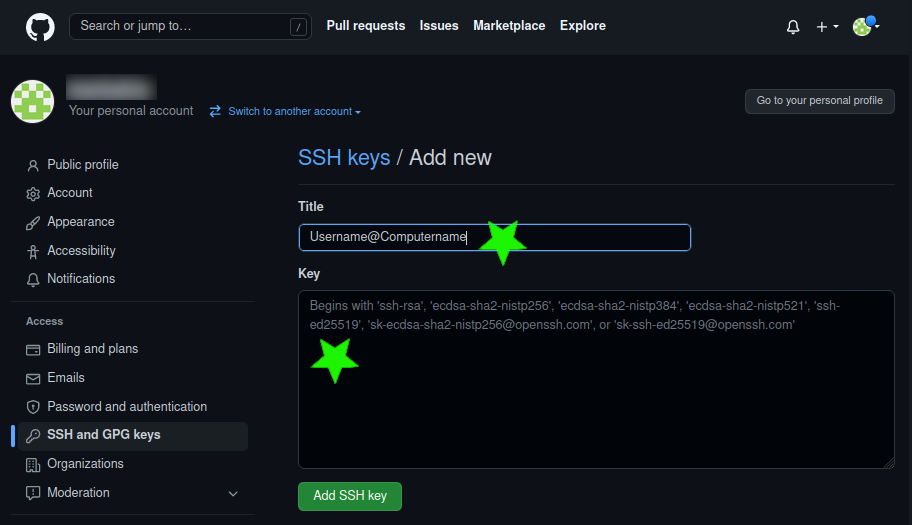
\includegraphics{Images/GH_04.png}
\caption{GitHub Step 4}
\end{figure}
\FloatBarrier

\begin{center}\rule{0.5\linewidth}{0.5pt}\end{center}

You'll also need to configure \texttt{git} on your computer as well.
Assuming you have \texttt{git} already installed, you can begin with
setting some of the initial variables.

You can configure individual repositories (projects) with these
settings, or you can configure \texttt{git} globally to set your
defaults. For now, we'll assume that you only have one GitHub account to
manage on your computer.

\begin{Shaded}
\begin{Highlighting}[]
\FunctionTok{git}\NormalTok{ config }\AttributeTok{{-}{-}global}\NormalTok{ user.name }\StringTok{"Firstname Lastname"}
\FunctionTok{git}\NormalTok{ config }\AttributeTok{{-}{-}global}\NormalTok{ user.email }\StringTok{"username@emailserver.com"}
\FunctionTok{git}\NormalTok{ config }\AttributeTok{{-}{-}global}\NormalTok{ user.user }\StringTok{"github\_username"}
\end{Highlighting}
\end{Shaded}

This next command may not mean too much right now, but it's useful to
have right off the bat to keep things clean later on.

\begin{Shaded}
\begin{Highlighting}[]
\FunctionTok{git}\NormalTok{ config }\AttributeTok{{-}{-}global}\NormalTok{ core.excludesFile }\StringTok{\textquotesingle{}\textasciitilde{}/.gitignore\textquotesingle{}}
\FunctionTok{touch}\NormalTok{ \textasciitilde{}/.gitignore}
\end{Highlighting}
\end{Shaded}

This tells git to ignore anything listed in the file
\texttt{\textasciitilde{}/.gitignore} when maintaining version controls.
This is useful for things like cached files produced by various Python
scripts, compiled programs/object files from C++, and so forth. As we
continue forward, we'll add some things to the global ignore, and others
to repository-specific \texttt{.gitignore} files.

\begin{center}\rule{0.5\linewidth}{0.5pt}\end{center}

Okay, we we've configured \texttt{git} on our computers, now how about
actually \emph{using} it?

Let's say you've made some headway on designing and maybe even coding up
some of your project, and you remember how important it is to maintain
version controls. You can initialize the project folder
\texttt{MyCodingProject} with the following command

\begin{Shaded}
\begin{Highlighting}[]
\FunctionTok{git}\NormalTok{ init MyCodingProject/}
\end{Highlighting}
\end{Shaded}

This establishes a starting point for all future versions to be compared
against.

For more useful commands, check out this cheat sheet!

\begin{figure}
\centering
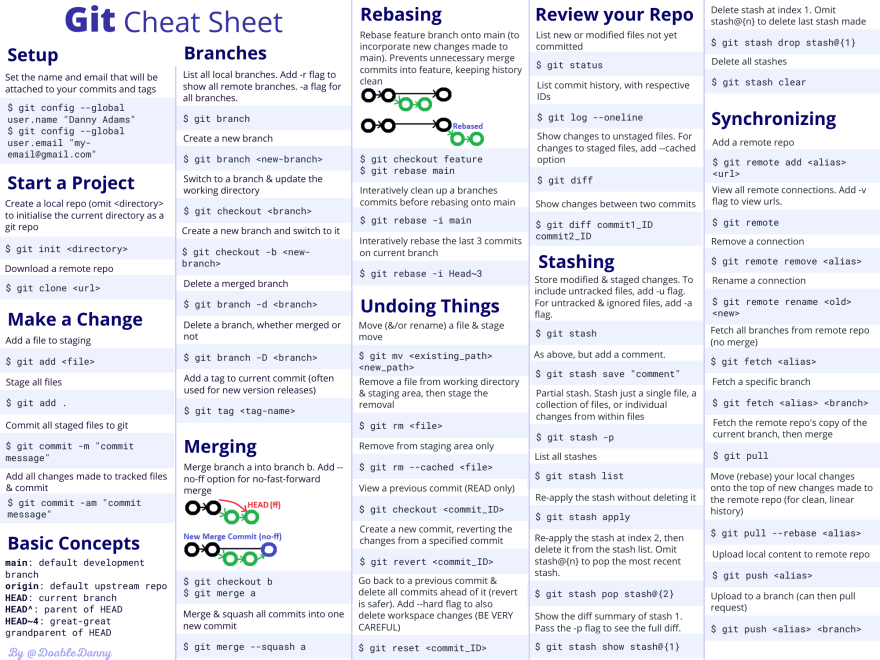
\includegraphics{Images/GitCheatSheet.png}
\caption{Git Cheat Sheet}
\end{figure}
\FloatBarrier

%%%%%%%%%%%%%%%%%%%%%%%%%%%%%%%%%%%%%%%%%%%%%%%%%%%%%%%%%%%%%%%%%%%%%%%%%%%%%%%%%%%%%%%%%%%%%%%%%%%%%%%%%%%%%%%%%%%%%
\section{Code Formatting}

Most programming languages have a form of something called
\textbf{scope}, which is a region in the code in which certain things
are true. For example, a function may have variables that only exist
inside that function, and then disappear once the program exits the
function's \textbf{scope}. Some languages use specific characters to
define a scope, such as \texttt{C++} with \texttt{\{} and \texttt{\}}
defining the beginning and end of a scope.

\begin{Shaded}
\begin{Highlighting}[]
\DataTypeTok{int}\NormalTok{ main}\OperatorTok{()}
\OperatorTok{\{}
\NormalTok{    cout }\OperatorTok{\textless{}\textless{}} \StringTok{"Hello World!}\SpecialCharTok{\textbackslash{}n}\StringTok{"}\OperatorTok{;}
    \ControlFlowTok{if} \OperatorTok{(}\DecValTok{5} \OperatorTok{\textless{}} \DecValTok{4}\OperatorTok{)}
    \OperatorTok{\{}
\NormalTok{        cout }\OperatorTok{\textless{}\textless{}} \StringTok{"Five is less than four.}\SpecialCharTok{\textbackslash{}n}\StringTok{"}\OperatorTok{;}
    \OperatorTok{\}}
    \ControlFlowTok{return}\OperatorTok{;}
\OperatorTok{\}}
\end{Highlighting}
\end{Shaded}

A common convention is to use spaces or tabs when moving into different
levels of scope, however this is usually for easier reading by humans
and isn't necessary for the code compiler itself.

Others, like \texttt{Python}, use indentations of spaces or tabs and are
specifically required to change scope.

\begin{Shaded}
\begin{Highlighting}[]
\KeywordTok{def}\NormalTok{ myfunction(x):}
\NormalTok{    x }\OperatorTok{=}\NormalTok{ x }\OperatorTok{+} \DecValTok{5}
    \BuiltInTok{print}\NormalTok{(x)}
    \ControlFlowTok{return}

\NormalTok{x }\OperatorTok{=} \DecValTok{10}
\BuiltInTok{print}\NormalTok{(x)}
\NormalTok{myfunction(x)}
\BuiltInTok{print}\NormalTok{(x)}
\end{Highlighting}
\end{Shaded}

The code snippet above shows the variable x inside the scope of
\texttt{myfunction} as well as the main program. If we follow the value
of \texttt{x} as the program runs, we can see that \texttt{x\ =\ 10},
which is printed out. Then, the \emph{value} of \texttt{x} is passed
into the function, which adds five and prints it out
(\texttt{x\ =\ 15}). Once that is done, the function returns, and the
main program's value of x is printed out again. (\texttt{x\ =\ 10}).

Let's see how that works in practice.

    \begin{tcolorbox}[breakable, size=fbox, boxrule=1pt, pad at break*=1mm,colback=cellbackground, colframe=cellborder]
\prompt{In}{incolor}{2}{\boxspacing}
\begin{Verbatim}[commandchars=\\\{\}]
\PY{k}{def} \PY{n+nf}{myfunction}\PY{p}{(}\PY{n}{x}\PY{p}{)}\PY{p}{:}
    \PY{n}{x} \PY{o}{=} \PY{n}{x} \PY{o}{+} \PY{l+m+mi}{5}
    \PY{n+nb}{print}\PY{p}{(}\PY{n}{x}\PY{p}{)}
    \PY{k}{return}

\PY{n}{x} \PY{o}{=} \PY{l+m+mi}{10}
\PY{n+nb}{print}\PY{p}{(}\PY{n}{x}\PY{p}{)}
\PY{n}{myfunction}\PY{p}{(}\PY{n}{x}\PY{p}{)}
\PY{n+nb}{print}\PY{p}{(}\PY{n}{x}\PY{p}{)}
\end{Verbatim}
\end{tcolorbox}

    \begin{Verbatim}[commandchars=\\\{\}]
10
15
10
    \end{Verbatim}

    It is very important to keep scope in mind when using variables as
counters or other housekeepers.

Many programmers use \texttt{i} as a counter variable in loops. However,
sometimes it is necessary to have loops inside other loops (nested),
which effectively means you have a scope inside another scope. If you
use \texttt{i} in the outer loop, then change it in the inner loop, it
remains changed in the outer loop and can have effects on the execution
of your code.

Therefore, it is important to keep track of what variables are used
during the execution of your code and how they are modified as you go.

\hypertarget{back-to-formatting}{%
\paragraph{Back to Formatting}\label{back-to-formatting}}

Formatting is not simply a matter of using indents or
80-characters-per-line requirements. Formatting also includes things
like expected code-comments or other internal documentation. Some code
development packages have the functionality built in to parse comments
in the code and build human-readable documentation, but it requires the
use of specific formats in the comments. See the examples below.

    \begin{tcolorbox}[breakable, size=fbox, boxrule=1pt, pad at break*=1mm,colback=cellbackground, colframe=cellborder]
\prompt{In}{incolor}{3}{\boxspacing}
\begin{Verbatim}[commandchars=\\\{\}]
\PY{k+kn}{import} \PY{n+nn}{numpy} \PY{k}{as} \PY{n+nn}{np}
\PY{k}{def} \PY{n+nf}{myfunction}\PY{p}{(}\PY{n}{x}\PY{p}{,}\PY{n}{y}\PY{p}{,}\PY{n}{z}\PY{p}{)}\PY{p}{:}
    \PY{n}{norm} \PY{o}{=} \PY{n}{np}\PY{o}{.}\PY{n}{linalg}\PY{o}{.}\PY{n}{norm}\PY{p}{(}\PY{p}{[}\PY{n}{x}\PY{p}{,}\PY{n}{y}\PY{p}{,}\PY{n}{z}\PY{p}{]}\PY{p}{)}
    \PY{k}{return} \PY{n}{norm}
\PY{n}{a} \PY{o}{=} \PY{l+m+mi}{1}
\PY{n}{b} \PY{o}{=} \PY{l+m+mi}{2}
\PY{n}{c} \PY{o}{=} \PY{l+m+mi}{3}
\PY{n}{result} \PY{o}{=} \PY{n}{myfunction}\PY{p}{(}\PY{n}{a}\PY{p}{,}\PY{n}{b}\PY{p}{,}\PY{n}{c}\PY{p}{)}
\PY{n+nb}{print}\PY{p}{(}\PY{n}{result}\PY{p}{)}
\end{Verbatim}
\end{tcolorbox}

    \begin{Verbatim}[commandchars=\\\{\}]
3.7416573867739413
    \end{Verbatim}

    The code block above has no comments in it, and so without already
knowing what the individual parts are doing, it's not easy to know what
is happening in the code or how to modify and manipulate it for your own
purposes. If we take the same code block and add some commentary, it can
be made easier.

    \begin{tcolorbox}[breakable, size=fbox, boxrule=1pt, pad at break*=1mm,colback=cellbackground, colframe=cellborder]
\prompt{In}{incolor}{4}{\boxspacing}
\begin{Verbatim}[commandchars=\\\{\}]
\PY{c+c1}{\PYZsh{} library import}
\PY{k+kn}{import} \PY{n+nn}{numpy} \PY{k}{as} \PY{n+nn}{np}

\PY{c+c1}{\PYZsh{} function definition}
\PY{k}{def} \PY{n+nf}{myfunction}\PY{p}{(}\PY{n}{x}\PY{p}{,}\PY{n}{y}\PY{p}{,}\PY{n}{z}\PY{p}{)}\PY{p}{:}
    \PY{n}{norm} \PY{o}{=} \PY{n}{np}\PY{o}{.}\PY{n}{linalg}\PY{o}{.}\PY{n}{norm}\PY{p}{(}\PY{p}{[}\PY{n}{x}\PY{p}{,}\PY{n}{y}\PY{p}{,}\PY{n}{z}\PY{p}{]}\PY{p}{)}
    \PY{k}{return} \PY{n}{norm}

\PY{c+c1}{\PYZsh{} Main program execution}
\PY{n}{a} \PY{o}{=} \PY{l+m+mi}{1}
\PY{n}{b} \PY{o}{=} \PY{l+m+mi}{2}
\PY{n}{c} \PY{o}{=} \PY{l+m+mi}{3}
\PY{n}{result} \PY{o}{=} \PY{n}{myfunction}\PY{p}{(}\PY{n}{a}\PY{p}{,}\PY{n}{b}\PY{p}{,}\PY{n}{c}\PY{p}{)}
\PY{n+nb}{print}\PY{p}{(}\PY{n}{result}\PY{p}{)}
\end{Verbatim}
\end{tcolorbox}

    \begin{Verbatim}[commandchars=\\\{\}]
3.7416573867739413
    \end{Verbatim}

    Now we have a little more clarity in what is happening, but it can still
be made clearer. As it stands, we simply know that we're importing
libraries, defining a function, and running the main program.

We can improve the commentary further by describing what is happening in
the function or the steps inside the main program.

    \begin{tcolorbox}[breakable, size=fbox, boxrule=1pt, pad at break*=1mm,colback=cellbackground, colframe=cellborder]
\prompt{In}{incolor}{5}{\boxspacing}
\begin{Verbatim}[commandchars=\\\{\}]
\PY{c+c1}{\PYZsh{} library import}
\PY{k+kn}{import} \PY{n+nn}{numpy} \PY{k}{as} \PY{n+nn}{np}

\PY{c+c1}{\PYZsh{} function definition}
\PY{k}{def} \PY{n+nf}{myfunction}\PY{p}{(}\PY{n}{x}\PY{p}{,}\PY{n}{y}\PY{p}{,}\PY{n}{z}\PY{p}{)}\PY{p}{:}
    \PY{c+c1}{\PYZsh{} Arguments:}
    \PY{c+c1}{\PYZsh{} x \PYZhy{} float representing the x component of a vector}
    \PY{c+c1}{\PYZsh{} y \PYZhy{} float representing the y component of a vector}
    \PY{c+c1}{\PYZsh{} z \PYZhy{} float representing the z component of a vector}
    \PY{c+c1}{\PYZsh{} Returns:}
    \PY{c+c1}{\PYZsh{} norm \PYZhy{} float representing the magnitude of the vector given by the [x,y,z] values}
    \PY{n}{norm} \PY{o}{=} \PY{n}{np}\PY{o}{.}\PY{n}{linalg}\PY{o}{.}\PY{n}{norm}\PY{p}{(}\PY{p}{[}\PY{n}{x}\PY{p}{,}\PY{n}{y}\PY{p}{,}\PY{n}{z}\PY{p}{]}\PY{p}{)}
    \PY{k}{return} \PY{n}{norm}

\PY{c+c1}{\PYZsh{} Main program execution}
\PY{c+c1}{\PYZsh{} initialize variables }
\PY{n}{a} \PY{o}{=} \PY{l+m+mi}{1}
\PY{n}{b} \PY{o}{=} \PY{l+m+mi}{2}
\PY{n}{c} \PY{o}{=} \PY{l+m+mi}{3}
\PY{c+c1}{\PYZsh{} obtain the magnitude of the vector defined by [a,b,c]}
\PY{n}{result} \PY{o}{=} \PY{n}{myfunction}\PY{p}{(}\PY{n}{a}\PY{p}{,}\PY{n}{b}\PY{p}{,}\PY{n}{c}\PY{p}{)}
\PY{c+c1}{\PYZsh{} print out the magnitude}
\PY{n+nb}{print}\PY{p}{(}\PY{n}{result}\PY{p}{)}
\end{Verbatim}
\end{tcolorbox}

    \begin{Verbatim}[commandchars=\\\{\}]
3.7416573867739413
    \end{Verbatim}

    With this level of commentary in the code, we can easily understand what
is happening in the function and the main code block. This is very
useful when working on collaborative projects especially, as it can
ensure that everyone is able to follow your thought process in the code
and, if necessary, compare to the actual code for debugging purposes.

Another thing to consider is the larger format of a project. That is,
not simply how the text is arranged in a file, but how code blocks and
functions are arranged in multiple files. For smaller programs, it may
not be necessary to divide the code up in this way, but for larger
projects - or for standard functions you'll use in multiple separate
projects - it may be easier and cleaner to keep some things separated
and compartmentalized. This also makes compiling easier later on down
the line.

It can also lead to smaller individual files, making debugging easier as
well - most error messages include the location where the error was
encountered, and it's much easier to go to
\texttt{line\ 46\ in\ utility.cpp} than it is to go to
\texttt{line\ 57684\ in\ main.cpp}. As a bonus, making changes in
smaller files won't necessarily require the entire codebase to be
recompiled, but rather just the small portion you modified.

%%%%%%%%%%%%%%%%%%%%%%%%%%%%%%%%%%%%%%%%%%%%%%%%%%%%%%%%%%%%%%%%%%%%%%%%%%%%%%%%%%%%%%%%%%%%%%%%%%%%%%%%%%%%%%%%%%%%%
\section{Debugging}
It's often said that only a small portion of programming is actually
writing the code - the rest is fixing the code.

Debugging is required at multiple stages of programming, and bugs can
arise in many different forms.

\hypertarget{compilation-bugs}{%
\paragraph{Compilation Bugs}\label{compilation-bugs}}

Compilation errors are usually the easiest to solve, as they're
encountered by the compiler itself and are often syntax-related
(``missing semicolon on line 85'') or datatype-related (``Unable to cast
string as int''), and usually include ``tracebacks'' which can help you
figure out where exactly the error is.

\hypertarget{runtime-bugs}{%
\paragraph{Runtime Bugs}\label{runtime-bugs}}

There are a few kinds of runtime errors that can pop up. They are
usually more complicated to unravel, depending on what caused them. The
first kind is something that, while the code will compile fine, the
actual execution will return an error. For example, a function that
takes \texttt{x} and \texttt{y} and returns the result of \texttt{x/y}
may compile just fine. But when you run the code, if somehow
\texttt{y\ =\ 0}, the program will crash because of an attempt to divide
by zero.

Another bug that can arise is when the results are not what was
expected. For instance, if you have a program that should return the
product of two numbers, and instead returns the sum of the two numbers,
this is a runtime error, even though no error is actually reported. The
code compiles fine and executes exactly as it is written, but it may not
be what was intended. These types of bugs are why validation and testing
are required for programs big and small.

Take a look at the code blocks below. One contains an example of a
compilation error, the other a runtime error.

    \begin{tcolorbox}[breakable, size=fbox, boxrule=1pt, pad at break*=1mm,colback=cellbackground, colframe=cellborder]
\prompt{In}{incolor}{7}{\boxspacing}
\begin{Verbatim}[commandchars=\\\{\}]
\PY{n+nb}{int} \PY{n}{x} \PY{o}{=} \PY{l+m+mi}{45}
\PY{n+nb}{print}\PY{p}{(}\PY{n}{x}\PY{p}{)}
\end{Verbatim}
\end{tcolorbox}

    \begin{Verbatim}[commandchars=\\\{\}, frame=single, framerule=2mm, rulecolor=\color{outerrorbackground}]
\textcolor{ansi-cyan}{  File }\textcolor{ansi-green}{"/tmp/ipykernel\_10751/2716038442.py"}\textcolor{ansi-cyan}{, line }\textcolor{ansi-green}{1}
\textcolor{ansi-red}{    int x = 45}
        \^{}
\textcolor{ansi-red}{SyntaxError}\textcolor{ansi-red}{:} invalid syntax

    \end{Verbatim}

    \begin{tcolorbox}[breakable, size=fbox, boxrule=1pt, pad at break*=1mm,colback=cellbackground, colframe=cellborder]
\prompt{In}{incolor}{10}{\boxspacing}
\begin{Verbatim}[commandchars=\\\{\}]
\PY{k}{def} \PY{n+nf}{divide}\PY{p}{(}\PY{n}{x}\PY{p}{,}\PY{n}{y}\PY{p}{)}\PY{p}{:}
    \PY{k}{return} \PY{n}{x}\PY{o}{/}\PY{n}{y}

\PY{n}{x} \PY{o}{=} \PY{l+m+mi}{5}
\PY{n}{y} \PY{o}{=} \PY{l+m+mi}{1}
\PY{n}{result} \PY{o}{=} \PY{n}{divide}\PY{p}{(}\PY{n}{x}\PY{p}{,}\PY{n}{y}\PY{p}{)}
\PY{n+nb}{print}\PY{p}{(}\PY{n}{x}\PY{p}{,}\PY{n}{y}\PY{p}{,}\PY{n}{result}\PY{p}{)}

\PY{n}{x} \PY{o}{=} \PY{l+m+mi}{5}
\PY{n}{y} \PY{o}{=} \PY{l+m+mi}{0}
\PY{n}{result} \PY{o}{=} \PY{n}{divide}\PY{p}{(}\PY{n}{x}\PY{p}{,}\PY{n}{y}\PY{p}{)}
\PY{n+nb}{print}\PY{p}{(}\PY{n}{x}\PY{p}{,}\PY{n}{y}\PY{p}{,}\PY{n}{result}\PY{p}{)}
\end{Verbatim}
\end{tcolorbox}

    \begin{Verbatim}[commandchars=\\\{\}]
5 1 5.0
    \end{Verbatim}

    \begin{Verbatim}[commandchars=\\\{\}, frame=single, framerule=2mm, rulecolor=\color{outerrorbackground}]
\textcolor{ansi-red}{---------------------------------------------------------------------------}
\textcolor{ansi-red}{ZeroDivisionError}                         Traceback (most recent call last)
\textcolor{ansi-green}{/tmp/ipykernel\_10751/1166490746.py} in \textcolor{ansi-cyan}{<module>}
\textcolor{ansi-green-intense}{\textbf{      9}} x \textcolor{ansi-blue}{=} \textcolor{ansi-cyan}{5}
\textcolor{ansi-green-intense}{\textbf{     10}} y \textcolor{ansi-blue}{=} \textcolor{ansi-cyan}{0}
\textcolor{ansi-green}{---> 11}\textcolor{ansi-red}{ }result \textcolor{ansi-blue}{=} divide\textcolor{ansi-blue}{(}x\textcolor{ansi-blue}{,}y\textcolor{ansi-blue}{)}
\textcolor{ansi-green-intense}{\textbf{     12}} print\textcolor{ansi-blue}{(}x\textcolor{ansi-blue}{,}y\textcolor{ansi-blue}{,}result\textcolor{ansi-blue}{)}
\textcolor{ansi-green-intense}{\textbf{     13}} 

\textcolor{ansi-green}{/tmp/ipykernel\_10751/1166490746.py} in \textcolor{ansi-cyan}{divide}\textcolor{ansi-blue}{(x, y)}
\textcolor{ansi-green-intense}{\textbf{      1}} \textcolor{ansi-green}{def} divide\textcolor{ansi-blue}{(}x\textcolor{ansi-blue}{,}y\textcolor{ansi-blue}{)}\textcolor{ansi-blue}{:}
\textcolor{ansi-green}{----> 2}\textcolor{ansi-red}{     }\textcolor{ansi-green}{return} x\textcolor{ansi-blue}{/}y
\textcolor{ansi-green-intense}{\textbf{      3}} 
\textcolor{ansi-green-intense}{\textbf{      4}} x \textcolor{ansi-blue}{=} \textcolor{ansi-cyan}{5}
\textcolor{ansi-green-intense}{\textbf{      5}} y \textcolor{ansi-blue}{=} \textcolor{ansi-cyan}{1}

\textcolor{ansi-red}{ZeroDivisionError}: division by zero
    \end{Verbatim}

    It should be pointed out that \emph{technically}, \texttt{Python}
doesn't have compile errors since it's not compiled at all, but runs
like a scripting language which merely interprets the commands line by
line. However, more advanced python programming can include the actual
compilation of python scripts into self-contained programs that don't
require any external libraries. This is not in the scope of this
workshop, however, and is merely pointed out for information.
%%%%%%%%%%%%%%%%%%%%%%%%%%%%%%%%%%%%%%%%%%%%%%%%%%%%%%%%%%%%%%%%%%%%%%%%%%%%%%%%%%%%%%%%%%%%%%%%%%%%%%%%%%%%%%%%%%%%%
\section{Pseudocode}
One of the most valuable skills a programmer can develop is the ability
to think like a computer. This means learning to break down larger
problems and complex behaviors into smaller and smaller pieces until it
becomes a collection of tiny calculations such as a sequence of
additions and subtractions, or comparisons between two values.

A good habit to develop whenever beginning a new project is to first
outline the expected flow of the code. Some people use a whiteboard, or
scratch paper, or just a blank text document on their computer - it
doesn't matter how you do it, just that you plan it out somehow before
jumping into the code.

\hypertarget{example-project---brownian-motion}{%
\paragraph{Example Project - Brownian
Motion}\label{example-project---brownian-motion}}

Write a program that places an arbitrary number of particles in a box of
some other arbitrary size, then moves them around randomly by assigning
a random x, y, and z component of their motion vector between 0 and 1.

Enter your pseudocode below. You can make it as complex as you like, but
it should just be plain text. Try to think through the steps of the
problem like a computer might.

\begin{center}\rule{0.5\linewidth}{0.5pt}\end{center}

    \textless!--- Pseudocode goes below

    \begin{center}\rule{0.5\linewidth}{0.5pt}\end{center}

Once you've completed your pseudocode, keep it handy - you can use it
for tomorrow's project!

%%%%%%%%%%%%%%%%%%%%%%%%%%%%%%%%%%%%%%%%%%%%%%%%%%%%%%%%%%%%%%%%%%%%%%%%%%%%%%%%%%%%%%%%%%%%%%%%%%%%%%%%%%%%%%%%%%%%%
\section{Data and Variable Types}
Python doesn't generally require \emph{explicit} variable type
declarations (with some exceptions that will come later as we get into
more advanced programming). However, it is still useful to know what
kinds of data there is, what can be done with it, and how it's stored.

First, let's explore data types like \texttt{int}, \texttt{float},
\texttt{list}, \texttt{tuple}, and \texttt{string}.

    \begin{tcolorbox}[breakable, size=fbox, boxrule=1pt, pad at break*=1mm,colback=cellbackground, colframe=cellborder]
\prompt{In}{incolor}{1}{\boxspacing}
\begin{Verbatim}[commandchars=\\\{\}]
\PY{n}{my\PYZus{}int}    \PY{o}{=} \PY{l+m+mi}{2}
\PY{n}{my\PYZus{}float}  \PY{o}{=} \PY{l+m+mf}{3.1415}
\PY{n}{my\PYZus{}list}   \PY{o}{=} \PY{p}{[}\PY{l+m+mi}{1}\PY{p}{,}\PY{l+m+mf}{3.1415}\PY{p}{,}\PY{l+s+s2}{\PYZdq{}}\PY{l+s+s2}{Hello World!}\PY{l+s+s2}{\PYZdq{}}\PY{p}{,}\PY{l+s+s2}{\PYZdq{}}\PY{l+s+s2}{pizza}\PY{l+s+s2}{\PYZdq{}}\PY{p}{]}
\PY{n}{my\PYZus{}tuple}  \PY{o}{=} \PY{p}{(}\PY{l+m+mi}{5}\PY{p}{,}\PY{l+m+mi}{6}\PY{p}{,}\PY{l+m+mi}{7}\PY{p}{,}\PY{l+m+mi}{8}\PY{p}{,}\PY{l+m+mi}{9}\PY{p}{)}
\PY{n}{my\PYZus{}string} \PY{o}{=} \PY{l+s+s2}{\PYZdq{}}\PY{l+s+s2}{Hello World!}\PY{l+s+s2}{\PYZdq{}}
\end{Verbatim}
\end{tcolorbox}

    These examples are fairly simple.

\begin{itemize}
\tightlist
\item
  \texttt{my\_int} is an integer, and gets treated like one. Integers
  are useful for things like indexes, counters, and so forth.
\item
  \texttt{my\_float} is a float (often called a ``double'' in other
  programming languages), and are regular numbers including decimals.
\item
  \texttt{my\_list} is a list of values enclosed in square brackets.
  Lists are indexed from zero, which means the first item in a list is
  ``item 0''. Lists are great ways to keep collections of data organized
  and in order, and you can extract individual values simply by
  including the index with the variable name: \texttt{my\_list{[}3{]}}
  will return ``pizza''. You can also get values from the end of a list
  with negative indices. my\_list\texttt{{[}-1{]}} will return ``pizza''
  because it's the last value.
\item
  \texttt{my\_tuple} is similar to a list, except that it is a little
  more difficult to pull individual values from it. Tuples are useful
  when you need to maintain groups of values together in relation to
  each other, such as with (x,y,z) coordinates.
\item
  \texttt{my\_string} is a list of characters including letters,
  numbers, punctuation, whitespace (tabs, spaces, line breaks, etc.).
  The contents of a string do not include the quotation marks on either
  side. Strings can include quotes using \emph{escapes} like
  \texttt{\textbackslash{}"} or
  \texttt{\textbackslash{}\textbackslash{}} to include a backslash.
\end{itemize}

Variable manipulation comes in many forms and depends on the type of
data contained within. Better understanding of how data types work can
allow you to do some interesting things, like taking a ``slice'' of a
string like you would from a list.

Consider the examples below.

    \begin{tcolorbox}[breakable, size=fbox, boxrule=1pt, pad at break*=1mm,colback=cellbackground, colframe=cellborder]
\prompt{In}{incolor}{2}{\boxspacing}
\begin{Verbatim}[commandchars=\\\{\}]
\PY{n}{my\PYZus{}list} \PY{o}{=} \PY{p}{[}\PY{l+m+mi}{0}\PY{p}{,}\PY{l+m+mi}{1}\PY{p}{,}\PY{l+m+mi}{2}\PY{p}{,}\PY{l+m+mi}{3}\PY{p}{,}\PY{l+m+mi}{4}\PY{p}{,}\PY{l+m+mi}{5}\PY{p}{,}\PY{l+m+mi}{6}\PY{p}{,}\PY{l+m+mi}{7}\PY{p}{,}\PY{l+m+mi}{8}\PY{p}{,}\PY{l+m+mi}{9}\PY{p}{,}\PY{l+m+mi}{10}\PY{p}{,}\PY{l+m+mi}{11}\PY{p}{,}\PY{l+m+mi}{12}\PY{p}{,}\PY{l+m+mi}{13}\PY{p}{,}\PY{l+m+mi}{14}\PY{p}{,}\PY{l+m+mi}{15}\PY{p}{,}\PY{l+m+mi}{16}\PY{p}{,}\PY{l+m+mi}{17}\PY{p}{,}\PY{l+m+mi}{18}\PY{p}{,}\PY{l+m+mi}{19}\PY{p}{,}\PY{l+m+mi}{20}\PY{p}{,}\PY{l+m+mi}{21}\PY{p}{,}\PY{l+m+mi}{22}\PY{p}{,}\PY{l+m+mi}{23}\PY{p}{,}\PY{l+m+mi}{24}\PY{p}{,}\PY{l+m+mi}{25}\PY{p}{]}
\PY{c+c1}{\PYZsh{} my\PYZus{}list has a length of 26 individual values}
\PY{n+nb}{len}\PY{p}{(}\PY{n}{my\PYZus{}list}\PY{p}{)}
\end{Verbatim}
\end{tcolorbox}

            \begin{tcolorbox}[breakable, size=fbox, boxrule=.5pt, pad at break*=1mm, opacityfill=0]
\prompt{Out}{outcolor}{2}{\boxspacing}
\begin{Verbatim}[commandchars=\\\{\}]
26
\end{Verbatim}
\end{tcolorbox}
        
    \begin{tcolorbox}[breakable, size=fbox, boxrule=1pt, pad at break*=1mm,colback=cellbackground, colframe=cellborder]
\prompt{In}{incolor}{3}{\boxspacing}
\begin{Verbatim}[commandchars=\\\{\}]
\PY{n}{my\PYZus{}string} \PY{o}{=} \PY{l+s+s2}{\PYZdq{}}\PY{l+s+s2}{Once more into the breach!}\PY{l+s+s2}{\PYZdq{}}
\PY{c+c1}{\PYZsh{} my\PYZus{}string has a length of 26 characters including whitespace and punctuation.}
\PY{n+nb}{len}\PY{p}{(}\PY{n}{my\PYZus{}string}\PY{p}{)}
\end{Verbatim}
\end{tcolorbox}

            \begin{tcolorbox}[breakable, size=fbox, boxrule=.5pt, pad at break*=1mm, opacityfill=0]
\prompt{Out}{outcolor}{3}{\boxspacing}
\begin{Verbatim}[commandchars=\\\{\}]
26
\end{Verbatim}
\end{tcolorbox}
        
    \hypertarget{slicing-lists}{%
\subsubsection{Slicing Lists}\label{slicing-lists}}

One common use for lists is ``slicing'', where you can get a small
subsection of the list. Let's say you wanted just the first five
elements in \texttt{my\_list}. You would use a slice. Slices are
generated similar to how an individual element is called from a list,
from inside square brackets. However, we can put a \texttt{:} between
the starting and ending indices to get everything between. We can also
use an empty space to indicate ``everything''. Check out the examples
below.

    \begin{tcolorbox}[breakable, size=fbox, boxrule=1pt, pad at break*=1mm,colback=cellbackground, colframe=cellborder]
\prompt{In}{incolor}{4}{\boxspacing}
\begin{Verbatim}[commandchars=\\\{\}]
\PY{n}{my\PYZus{}list}\PY{p}{[}\PY{p}{:}\PY{l+m+mi}{5}\PY{p}{]}
\end{Verbatim}
\end{tcolorbox}

            \begin{tcolorbox}[breakable, size=fbox, boxrule=.5pt, pad at break*=1mm, opacityfill=0]
\prompt{Out}{outcolor}{4}{\boxspacing}
\begin{Verbatim}[commandchars=\\\{\}]
[0, 1, 2, 3, 4]
\end{Verbatim}
\end{tcolorbox}
        
    \begin{tcolorbox}[breakable, size=fbox, boxrule=1pt, pad at break*=1mm,colback=cellbackground, colframe=cellborder]
\prompt{In}{incolor}{5}{\boxspacing}
\begin{Verbatim}[commandchars=\\\{\}]
\PY{n}{my\PYZus{}list}\PY{p}{[}\PY{l+m+mi}{5}\PY{p}{:}\PY{l+m+mi}{10}\PY{p}{]}
\end{Verbatim}
\end{tcolorbox}

            \begin{tcolorbox}[breakable, size=fbox, boxrule=.5pt, pad at break*=1mm, opacityfill=0]
\prompt{Out}{outcolor}{5}{\boxspacing}
\begin{Verbatim}[commandchars=\\\{\}]
[5, 6, 7, 8, 9]
\end{Verbatim}
\end{tcolorbox}
        
    Note how the two results are different. The ending in the first cell is
the same as the beginning of the second cell, but we don't actually get
``5'' in the results in the first cell. Slices go ``up to'' the ending
value, but don't include it. Keep this in mind when working with slices.
We can also combine other tricks from list manipulations, like using
negative indices to go backwards from the end.

In the next cell, we'll get the last seven elements from the list.

    \begin{tcolorbox}[breakable, size=fbox, boxrule=1pt, pad at break*=1mm,colback=cellbackground, colframe=cellborder]
\prompt{In}{incolor}{6}{\boxspacing}
\begin{Verbatim}[commandchars=\\\{\}]
\PY{n}{my\PYZus{}list}\PY{p}{[}\PY{o}{\PYZhy{}}\PY{l+m+mi}{7}\PY{p}{:}\PY{p}{]}
\end{Verbatim}
\end{tcolorbox}

            \begin{tcolorbox}[breakable, size=fbox, boxrule=.5pt, pad at break*=1mm, opacityfill=0]
\prompt{Out}{outcolor}{6}{\boxspacing}
\begin{Verbatim}[commandchars=\\\{\}]
[19, 20, 21, 22, 23, 24, 25]
\end{Verbatim}
\end{tcolorbox}
        
    What if we wanted every third element in the list?

    \begin{tcolorbox}[breakable, size=fbox, boxrule=1pt, pad at break*=1mm,colback=cellbackground, colframe=cellborder]
\prompt{In}{incolor}{7}{\boxspacing}
\begin{Verbatim}[commandchars=\\\{\}]
\PY{n}{my\PYZus{}list}\PY{p}{[}\PY{p}{:}\PY{p}{:}\PY{l+m+mi}{3}\PY{p}{]}
\end{Verbatim}
\end{tcolorbox}

            \begin{tcolorbox}[breakable, size=fbox, boxrule=.5pt, pad at break*=1mm, opacityfill=0]
\prompt{Out}{outcolor}{7}{\boxspacing}
\begin{Verbatim}[commandchars=\\\{\}]
[0, 3, 6, 9, 12, 15, 18, 21, 24]
\end{Verbatim}
\end{tcolorbox}
        
    The second \texttt{:} indicates a ``stride''. This is useful when you
have data that is strangely shaped (such as a long list of values that
correspond to x,y,z coordinates, but aren't in a (3,n) shaped list.

Now let's combine these. We'll get every other element starting from the
tenth and going up to the twentieth.

    \begin{tcolorbox}[breakable, size=fbox, boxrule=1pt, pad at break*=1mm,colback=cellbackground, colframe=cellborder]
\prompt{In}{incolor}{8}{\boxspacing}
\begin{Verbatim}[commandchars=\\\{\}]
\PY{n}{my\PYZus{}list}\PY{p}{[}\PY{l+m+mi}{10}\PY{p}{:}\PY{l+m+mi}{20}\PY{p}{:}\PY{l+m+mi}{2}\PY{p}{]}
\end{Verbatim}
\end{tcolorbox}

            \begin{tcolorbox}[breakable, size=fbox, boxrule=.5pt, pad at break*=1mm, opacityfill=0]
\prompt{Out}{outcolor}{8}{\boxspacing}
\begin{Verbatim}[commandchars=\\\{\}]
[10, 12, 14, 16, 18]
\end{Verbatim}
\end{tcolorbox}
        
    Now let's look at strings. Strings are just lists of letters, numbers,
and any other characters you can think of. With this in mind, we can do
things to strings that we have done to lists.

    \begin{tcolorbox}[breakable, size=fbox, boxrule=1pt, pad at break*=1mm,colback=cellbackground, colframe=cellborder]
\prompt{In}{incolor}{9}{\boxspacing}
\begin{Verbatim}[commandchars=\\\{\}]
\PY{n}{my\PYZus{}string}
\end{Verbatim}
\end{tcolorbox}

            \begin{tcolorbox}[breakable, size=fbox, boxrule=.5pt, pad at break*=1mm, opacityfill=0]
\prompt{Out}{outcolor}{9}{\boxspacing}
\begin{Verbatim}[commandchars=\\\{\}]
'Once more into the breach!'
\end{Verbatim}
\end{tcolorbox}
        
    \begin{tcolorbox}[breakable, size=fbox, boxrule=1pt, pad at break*=1mm,colback=cellbackground, colframe=cellborder]
\prompt{In}{incolor}{10}{\boxspacing}
\begin{Verbatim}[commandchars=\\\{\}]
\PY{n}{my\PYZus{}string}\PY{p}{[}\PY{p}{:}\PY{l+m+mi}{5}\PY{p}{]}
\end{Verbatim}
\end{tcolorbox}

            \begin{tcolorbox}[breakable, size=fbox, boxrule=.5pt, pad at break*=1mm, opacityfill=0]
\prompt{Out}{outcolor}{10}{\boxspacing}
\begin{Verbatim}[commandchars=\\\{\}]
'Once '
\end{Verbatim}
\end{tcolorbox}
        
    \begin{tcolorbox}[breakable, size=fbox, boxrule=1pt, pad at break*=1mm,colback=cellbackground, colframe=cellborder]
\prompt{In}{incolor}{11}{\boxspacing}
\begin{Verbatim}[commandchars=\\\{\}]
\PY{n}{my\PYZus{}string}\PY{p}{[}\PY{l+m+mi}{5}\PY{p}{:}\PY{l+m+mi}{10}\PY{p}{]}
\end{Verbatim}
\end{tcolorbox}

            \begin{tcolorbox}[breakable, size=fbox, boxrule=.5pt, pad at break*=1mm, opacityfill=0]
\prompt{Out}{outcolor}{11}{\boxspacing}
\begin{Verbatim}[commandchars=\\\{\}]
'more '
\end{Verbatim}
\end{tcolorbox}
        
    \begin{tcolorbox}[breakable, size=fbox, boxrule=1pt, pad at break*=1mm,colback=cellbackground, colframe=cellborder]
\prompt{In}{incolor}{12}{\boxspacing}
\begin{Verbatim}[commandchars=\\\{\}]
\PY{n}{my\PYZus{}string}\PY{p}{[}\PY{o}{\PYZhy{}}\PY{l+m+mi}{7}\PY{p}{:}\PY{p}{]}
\end{Verbatim}
\end{tcolorbox}

            \begin{tcolorbox}[breakable, size=fbox, boxrule=.5pt, pad at break*=1mm, opacityfill=0]
\prompt{Out}{outcolor}{12}{\boxspacing}
\begin{Verbatim}[commandchars=\\\{\}]
'breach!'
\end{Verbatim}
\end{tcolorbox}
        
    \begin{tcolorbox}[breakable, size=fbox, boxrule=1pt, pad at break*=1mm,colback=cellbackground, colframe=cellborder]
\prompt{In}{incolor}{13}{\boxspacing}
\begin{Verbatim}[commandchars=\\\{\}]
\PY{n}{my\PYZus{}string}\PY{p}{[}\PY{p}{:}\PY{p}{:}\PY{l+m+mi}{3}\PY{p}{]}
\end{Verbatim}
\end{tcolorbox}

            \begin{tcolorbox}[breakable, size=fbox, boxrule=.5pt, pad at break*=1mm, opacityfill=0]
\prompt{Out}{outcolor}{13}{\boxspacing}
\begin{Verbatim}[commandchars=\\\{\}]
'Oeo tt eh'
\end{Verbatim}
\end{tcolorbox}
        
    \begin{tcolorbox}[breakable, size=fbox, boxrule=1pt, pad at break*=1mm,colback=cellbackground, colframe=cellborder]
\prompt{In}{incolor}{14}{\boxspacing}
\begin{Verbatim}[commandchars=\\\{\}]
\PY{n}{my\PYZus{}string}\PY{p}{[}\PY{l+m+mi}{10}\PY{p}{:}\PY{l+m+mi}{20}\PY{p}{:}\PY{l+m+mi}{2}\PY{p}{]}
\end{Verbatim}
\end{tcolorbox}

            \begin{tcolorbox}[breakable, size=fbox, boxrule=.5pt, pad at break*=1mm, opacityfill=0]
\prompt{Out}{outcolor}{14}{\boxspacing}
\begin{Verbatim}[commandchars=\\\{\}]
'it h '
\end{Verbatim}
\end{tcolorbox}
        
    \ldots{} some functions are more useful than others, but you get the
idea!

Now let's look at integers and floats. In some programming languages,
the difference between these two can be pretty severe. For example, in
C++, dividing a double by an integer will give you a truncated integer,
which means you can lose some of the information in your data if you're
not careful. Thankfully, Python is a little more forgiving.

Normal division works like we might intuitively expect, where a float
divided by an integer can be a float, and is therefore assumed to be.

    \begin{tcolorbox}[breakable, size=fbox, boxrule=1pt, pad at break*=1mm,colback=cellbackground, colframe=cellborder]
\prompt{In}{incolor}{15}{\boxspacing}
\begin{Verbatim}[commandchars=\\\{\}]
\PY{n}{my\PYZus{}float}\PY{o}{/}\PY{n}{my\PYZus{}int}
\end{Verbatim}
\end{tcolorbox}

            \begin{tcolorbox}[breakable, size=fbox, boxrule=.5pt, pad at break*=1mm, opacityfill=0]
\prompt{Out}{outcolor}{15}{\boxspacing}
\begin{Verbatim}[commandchars=\\\{\}]
1.57075
\end{Verbatim}
\end{tcolorbox}
        
    We can also force the division to return an integer value (which is
useful in some situations)

In the example above, we got a value of 1.57075. If we were to round
this using conventional methods, we'd get 2 However, forcing integer
division with the \texttt{//} below gives us a truncated (not rounded)
value of 1.0. This is also slightly deceptive, as the \texttt{.0}
implies the value is a float,even though the result is a whole number.
This is important to be aware of when doing mathematical work in python.
Truncation just removes everything after the decimal point, while
rounding actually considers the value beforehand.

    \begin{tcolorbox}[breakable, size=fbox, boxrule=1pt, pad at break*=1mm,colback=cellbackground, colframe=cellborder]
\prompt{In}{incolor}{16}{\boxspacing}
\begin{Verbatim}[commandchars=\\\{\}]
\PY{n}{my\PYZus{}float}\PY{o}{/}\PY{o}{/}\PY{n}{my\PYZus{}int}
\end{Verbatim}
\end{tcolorbox}

            \begin{tcolorbox}[breakable, size=fbox, boxrule=.5pt, pad at break*=1mm, opacityfill=0]
\prompt{Out}{outcolor}{16}{\boxspacing}
\begin{Verbatim}[commandchars=\\\{\}]
1.0
\end{Verbatim}
\end{tcolorbox}
        
    \begin{tcolorbox}[breakable, size=fbox, boxrule=1pt, pad at break*=1mm,colback=cellbackground, colframe=cellborder]
\prompt{In}{incolor}{17}{\boxspacing}
\begin{Verbatim}[commandchars=\\\{\}]
\PY{n+nb}{round}\PY{p}{(}\PY{n}{my\PYZus{}float}\PY{o}{/}\PY{n}{my\PYZus{}int}\PY{p}{)}
\end{Verbatim}
\end{tcolorbox}

            \begin{tcolorbox}[breakable, size=fbox, boxrule=.5pt, pad at break*=1mm, opacityfill=0]
\prompt{Out}{outcolor}{17}{\boxspacing}
\begin{Verbatim}[commandchars=\\\{\}]
2
\end{Verbatim}
\end{tcolorbox}
        
    \hypertarget{math-with-variables}{%
\subsubsection{Math with Variables}\label{math-with-variables}}

Math can get incredibly complex, so it's important to remember your
Order of Operations (PEMDAS) - Parentheses, Exponents, Multiplication,
Division, Addition, and Subtraction.

However, in python it's a little different. Parentheses are solved
first, then exponents, until everything in a given equation is reduced
down to a series of terms separated by \texttt{+},\texttt{-},\texttt{*},
and \texttt{/}. Then, the values are processed left-to-right.

    \begin{tcolorbox}[breakable, size=fbox, boxrule=1pt, pad at break*=1mm,colback=cellbackground, colframe=cellborder]
\prompt{In}{incolor}{18}{\boxspacing}
\begin{Verbatim}[commandchars=\\\{\}]
\PY{l+m+mi}{1} \PY{o}{+} \PY{l+m+mi}{2} \PY{o}{\PYZhy{}} \PY{l+m+mi}{3} \PY{o}{*} \PY{l+m+mi}{4} \PY{o}{/} \PY{l+m+mi}{5}
\end{Verbatim}
\end{tcolorbox}

            \begin{tcolorbox}[breakable, size=fbox, boxrule=.5pt, pad at break*=1mm, opacityfill=0]
\prompt{Out}{outcolor}{18}{\boxspacing}
\begin{Verbatim}[commandchars=\\\{\}]
0.6000000000000001
\end{Verbatim}
\end{tcolorbox}
        
    \begin{tcolorbox}[breakable, size=fbox, boxrule=1pt, pad at break*=1mm,colback=cellbackground, colframe=cellborder]
\prompt{In}{incolor}{19}{\boxspacing}
\begin{Verbatim}[commandchars=\\\{\}]
\PY{p}{(}\PY{l+m+mi}{1} \PY{o}{+} \PY{l+m+mi}{2}\PY{p}{)} \PY{o}{\PYZhy{}} \PY{l+m+mi}{3} \PY{o}{*} \PY{l+m+mi}{4} \PY{o}{/} \PY{l+m+mi}{5}
\end{Verbatim}
\end{tcolorbox}

            \begin{tcolorbox}[breakable, size=fbox, boxrule=.5pt, pad at break*=1mm, opacityfill=0]
\prompt{Out}{outcolor}{19}{\boxspacing}
\begin{Verbatim}[commandchars=\\\{\}]
0.6000000000000001
\end{Verbatim}
\end{tcolorbox}
        
    \begin{tcolorbox}[breakable, size=fbox, boxrule=1pt, pad at break*=1mm,colback=cellbackground, colframe=cellborder]
\prompt{In}{incolor}{20}{\boxspacing}
\begin{Verbatim}[commandchars=\\\{\}]
\PY{p}{(}\PY{l+m+mi}{1} \PY{o}{+} \PY{l+m+mi}{2} \PY{o}{\PYZhy{}} \PY{l+m+mi}{3} \PY{o}{*} \PY{l+m+mi}{4}\PY{p}{)} \PY{o}{/} \PY{l+m+mi}{5}
\end{Verbatim}
\end{tcolorbox}

            \begin{tcolorbox}[breakable, size=fbox, boxrule=.5pt, pad at break*=1mm, opacityfill=0]
\prompt{Out}{outcolor}{20}{\boxspacing}
\begin{Verbatim}[commandchars=\\\{\}]
-1.8
\end{Verbatim}
\end{tcolorbox}
        
    \begin{tcolorbox}[breakable, size=fbox, boxrule=1pt, pad at break*=1mm,colback=cellbackground, colframe=cellborder]
\prompt{In}{incolor}{21}{\boxspacing}
\begin{Verbatim}[commandchars=\\\{\}]
\PY{p}{(}\PY{l+m+mi}{1} \PY{o}{+} \PY{l+m+mi}{2} \PY{o}{\PYZhy{}} \PY{l+m+mi}{3}\PY{p}{)} \PY{o}{*} \PY{l+m+mi}{4} \PY{o}{/} \PY{l+m+mi}{5}
\end{Verbatim}
\end{tcolorbox}

            \begin{tcolorbox}[breakable, size=fbox, boxrule=.5pt, pad at break*=1mm, opacityfill=0]
\prompt{Out}{outcolor}{21}{\boxspacing}
\begin{Verbatim}[commandchars=\\\{\}]
0.0
\end{Verbatim}
\end{tcolorbox}
        
    These are just a few examples of how order of operations affects the
results. With this in mind, you can see why it's very important to keep
track of what you're doing in a complex mathematical function. The next
cell has a complex equation in a single line, then the same equation
separated into more easily-managed terms.

    \begin{tcolorbox}[breakable, size=fbox, boxrule=1pt, pad at break*=1mm,colback=cellbackground, colframe=cellborder]
\prompt{In}{incolor}{22}{\boxspacing}
\begin{Verbatim}[commandchars=\\\{\}]
\PY{n}{x}\PY{o}{=}\PY{l+m+mi}{3}
\PY{n}{y}\PY{o}{=}\PY{l+m+mi}{5}
\PY{n}{z}\PY{o}{=}\PY{l+m+mi}{7}
\PY{n}{answer} \PY{o}{=}  \PY{p}{(}\PY{n}{x}\PY{o}{*}\PY{o}{*}\PY{p}{(}\PY{n}{y}\PY{o}{/}\PY{n}{z}\PY{p}{)}\PY{o}{\PYZhy{}}\PY{n}{x}\PY{o}{/}\PY{p}{(}\PY{p}{(}\PY{n}{y}\PY{o}{+}\PY{l+m+mi}{2}\PY{p}{)}\PY{o}{*}\PY{n}{z}\PY{p}{)}\PY{o}{\PYZhy{}}\PY{n}{x}\PY{p}{)}\PY{o}{/}\PY{p}{(}\PY{n}{y}\PY{o}{*}\PY{n}{z}\PY{p}{)}\PY{o}{*}\PY{n}{x}

\PY{n+nb}{print}\PY{p}{(}\PY{n}{answer}\PY{p}{)}
\end{Verbatim}
\end{tcolorbox}

    \begin{Verbatim}[commandchars=\\\{\}]
-0.07452211053138932
    \end{Verbatim}

    Not only is that difficult to read, but it's also harder to see where
errors might be arising. So we can rewrite it and create additional
variables to hold small chunks

    \begin{tcolorbox}[breakable, size=fbox, boxrule=1pt, pad at break*=1mm,colback=cellbackground, colframe=cellborder]
\prompt{In}{incolor}{23}{\boxspacing}
\begin{Verbatim}[commandchars=\\\{\}]
\PY{n}{x}\PY{o}{=}\PY{l+m+mi}{3}
\PY{n}{y}\PY{o}{=}\PY{l+m+mi}{5}
\PY{n}{z}\PY{o}{=}\PY{l+m+mi}{7}

\PY{c+c1}{\PYZsh{} (x**(y/z)\PYZhy{}x/((y+2)*z)\PYZhy{}x)/(y*z)*x}
\PY{n}{p} \PY{o}{=} \PY{n}{y}\PY{o}{/}\PY{n}{z}
\PY{c+c1}{\PYZsh{} (x**p\PYZhy{}x/((y+2)*z)\PYZhy{}x)/(y*z)*x}
\PY{n}{q} \PY{o}{=} \PY{n}{x}\PY{o}{*}\PY{o}{*}\PY{n}{p}
\PY{c+c1}{\PYZsh{} (q\PYZhy{}x/((y+2)*z)\PYZhy{}x)/(y*z)*x}
\PY{n}{r} \PY{o}{=} \PY{n}{y}\PY{o}{+}\PY{l+m+mi}{2}
\PY{c+c1}{\PYZsh{} (q\PYZhy{}x/(r*z)\PYZhy{}x)/(y*z)*x}
\PY{n}{s} \PY{o}{=} \PY{n}{r}\PY{o}{*}\PY{n}{z}
\PY{c+c1}{\PYZsh{} (q\PYZhy{}x/s\PYZhy{}x)/(y*z)*x}
\PY{n}{t} \PY{o}{=} \PY{n}{y}\PY{o}{*}\PY{n}{z}
\PY{c+c1}{\PYZsh{} (q\PYZhy{}x/s\PYZhy{}x)/t*x}
\PY{n}{u} \PY{o}{=} \PY{n}{x}\PY{o}{/}\PY{n}{s}
\PY{c+c1}{\PYZsh{} (q\PYZhy{}u\PYZhy{}x)/t*x}
\PY{n}{v} \PY{o}{=} \PY{n}{q}\PY{o}{\PYZhy{}}\PY{n}{u}\PY{o}{\PYZhy{}}\PY{n}{x}
\PY{c+c1}{\PYZsh{} v/t*x}
\PY{n}{w} \PY{o}{=} \PY{n}{v}\PY{o}{/}\PY{n}{t}
\PY{c+c1}{\PYZsh{} w*x}
\PY{n}{answer} \PY{o}{=} \PY{n}{w}\PY{o}{*}\PY{n}{x}

\PY{n+nb}{print}\PY{p}{(}\PY{n}{answer}\PY{p}{)}
\end{Verbatim}
\end{tcolorbox}

    \begin{Verbatim}[commandchars=\\\{\}]
-0.07452211053138932
    \end{Verbatim}

    This may seem overengineered, but breaking down the individual terms is
helpful in both programming and math, especially when it reveals certain
trends, or even ways to rearrange an equation to reduce the overall
number of calculations being performed. This kind of breakdown can also
be useful when you begin building larger, more complicated functions,
even up to the point of creating entire programs or modules.

\hypertarget{booleans}{%
\subsubsection{Booleans}\label{booleans}}

Booleans are simply variables that are either \texttt{True} or
\texttt{False}. They can also be interpreted as \texttt{1} and
\texttt{0}. Booleans get used all the time in programming, though we may
not be constantly aware of them.

For example, whenever we compare two numbers, the comparison creates a
boolean

    \begin{tcolorbox}[breakable, size=fbox, boxrule=1pt, pad at break*=1mm,colback=cellbackground, colframe=cellborder]
\prompt{In}{incolor}{24}{\boxspacing}
\begin{Verbatim}[commandchars=\\\{\}]
\PY{l+m+mi}{3}\PY{o}{\PYZlt{}}\PY{l+m+mi}{5}
\end{Verbatim}
\end{tcolorbox}

            \begin{tcolorbox}[breakable, size=fbox, boxrule=.5pt, pad at break*=1mm, opacityfill=0]
\prompt{Out}{outcolor}{24}{\boxspacing}
\begin{Verbatim}[commandchars=\\\{\}]
True
\end{Verbatim}
\end{tcolorbox}
        
    \begin{tcolorbox}[breakable, size=fbox, boxrule=1pt, pad at break*=1mm,colback=cellbackground, colframe=cellborder]
\prompt{In}{incolor}{25}{\boxspacing}
\begin{Verbatim}[commandchars=\\\{\}]
\PY{l+m+mi}{3}\PY{o}{\PYZgt{}}\PY{l+m+mi}{5}
\end{Verbatim}
\end{tcolorbox}

            \begin{tcolorbox}[breakable, size=fbox, boxrule=.5pt, pad at break*=1mm, opacityfill=0]
\prompt{Out}{outcolor}{25}{\boxspacing}
\begin{Verbatim}[commandchars=\\\{\}]
False
\end{Verbatim}
\end{tcolorbox}
        
    \begin{tcolorbox}[breakable, size=fbox, boxrule=1pt, pad at break*=1mm,colback=cellbackground, colframe=cellborder]
\prompt{In}{incolor}{26}{\boxspacing}
\begin{Verbatim}[commandchars=\\\{\}]
\PY{l+m+mi}{3} \PY{o}{==} \PY{l+m+mi}{5}
\end{Verbatim}
\end{tcolorbox}

            \begin{tcolorbox}[breakable, size=fbox, boxrule=.5pt, pad at break*=1mm, opacityfill=0]
\prompt{Out}{outcolor}{26}{\boxspacing}
\begin{Verbatim}[commandchars=\\\{\}]
False
\end{Verbatim}
\end{tcolorbox}
        
    We can see that the responses for the different comparisons are correct.
\(3 < 5\) is true, while \(3 > 5\) and \(3 == 5\) are both false.
Incidentally, the \texttt{==} is intentional. In Python and C++,
\texttt{=} \emph{assigns} a value, while \texttt{==} \emph{compares} two
values.

Booleans get used constantly in things like ``if-else statements'' or
``while loops''.

\hypertarget{dictionaries}{%
\subsubsection{Dictionaries}\label{dictionaries}}

Another python data type is the \texttt{dictionary} (or \texttt{dict} as
it's written in python). The dictionary is a very useful datatype, as it
can be used to store many different pieces of information in their own
types.

    \begin{tcolorbox}[breakable, size=fbox, boxrule=1pt, pad at break*=1mm,colback=cellbackground, colframe=cellborder]
\prompt{In}{incolor}{27}{\boxspacing}
\begin{Verbatim}[commandchars=\\\{\}]
\PY{c+c1}{\PYZsh{} A dictionary is denoted by \PYZob{} \PYZcb{} }
\PY{n}{my\PYZus{}dictionary} \PY{o}{=} \PY{p}{\PYZob{}}\PY{p}{\PYZcb{}}

\PY{c+c1}{\PYZsh{} At this point, \PYZdq{}my\PYZus{}dictionary\PYZdq{} is an empty dictionary with no keys or values assigned.}
\PY{c+c1}{\PYZsh{} We can assign a key/value pair like this}

\PY{n}{my\PYZus{}dictionary}\PY{p}{[}\PY{l+s+s2}{\PYZdq{}}\PY{l+s+s2}{Name}\PY{l+s+s2}{\PYZdq{}}\PY{p}{]} \PY{o}{=} \PY{l+s+s2}{\PYZdq{}}\PY{l+s+s2}{Mark}\PY{l+s+s2}{\PYZdq{}}
\PY{n}{my\PYZus{}dictionary}\PY{p}{[}\PY{l+s+s2}{\PYZdq{}}\PY{l+s+s2}{Age}\PY{l+s+s2}{\PYZdq{}}\PY{p}{]}  \PY{o}{=} \PY{l+m+mi}{37}
\PY{n}{my\PYZus{}dictionary}\PY{p}{[}\PY{l+s+s2}{\PYZdq{}}\PY{l+s+s2}{Job}\PY{l+s+s2}{\PYZdq{}}\PY{p}{]} \PY{o}{=} \PY{l+s+s2}{\PYZdq{}}\PY{l+s+s2}{Postdoc}\PY{l+s+s2}{\PYZdq{}}

\PY{c+c1}{\PYZsh{} Now we can recall any of the values held in the dictionary by using the [key]. Keep in mind, if a key already exists, the previous value will be overwritten.}

\PY{c+c1}{\PYZsh{} If you have a dictionary with keys that you don\PYZsq{}t know, you can get them like this:}
\PY{n}{key\PYZus{}list} \PY{o}{=} \PY{p}{[}\PY{n}{key} \PY{k}{for} \PY{n}{key} \PY{o+ow}{in} \PY{n}{my\PYZus{}dictionary}\PY{o}{.}\PY{n}{keys}\PY{p}{(}\PY{p}{)}\PY{p}{]}
\PY{n+nb}{print}\PY{p}{(}\PY{n}{key\PYZus{}list}\PY{p}{)}
\PY{c+c1}{\PYZsh{} This might look strange, but it\PYZsq{}s done this way because my\PYZus{}dictionary.keys() is a function call that returns an iterative set of single values, rather than the entire list.}

\PY{c+c1}{\PYZsh{} You can also iterate through all the keys and values together.}
\PY{k}{for} \PY{n}{key}\PY{p}{,}\PY{n}{value} \PY{o+ow}{in} \PY{n}{my\PYZus{}dictionary}\PY{o}{.}\PY{n}{items}\PY{p}{(}\PY{p}{)}\PY{p}{:}
    \PY{n+nb}{print}\PY{p}{(}\PY{n}{key}\PY{p}{,}\PY{l+s+s2}{\PYZdq{}}\PY{l+s+s2}{=}\PY{l+s+s2}{\PYZdq{}}\PY{p}{,}\PY{n}{value}\PY{p}{)}
\end{Verbatim}
\end{tcolorbox}

    \begin{Verbatim}[commandchars=\\\{\}]
['Name', 'Age', 'Job']
Name = Mark
Age = 37
Job = Postdoc
    \end{Verbatim}

    \begin{tcolorbox}[breakable, size=fbox, boxrule=1pt, pad at break*=1mm,colback=cellbackground, colframe=cellborder]
\prompt{In}{incolor}{28}{\boxspacing}
\begin{Verbatim}[commandchars=\\\{\}]
\PY{c+c1}{\PYZsh{} In a more relevant example to the lab (and demonstration of dictionary initialization with keys and values):}

\PY{n}{variant\PYZus{}prmtops} \PY{o}{=} \PY{p}{\PYZob{}}\PY{l+s+s2}{\PYZdq{}}\PY{l+s+s2}{WT}\PY{l+s+s2}{\PYZdq{}}\PY{p}{:}\PY{l+s+s2}{\PYZdq{}}\PY{l+s+s2}{A3H\PYZus{}WT.prmtop}\PY{l+s+s2}{\PYZdq{}}\PY{p}{,}
                   \PY{l+s+s2}{\PYZdq{}}\PY{l+s+s2}{K121E}\PY{l+s+s2}{\PYZdq{}}\PY{p}{:}\PY{l+s+s2}{\PYZdq{}}\PY{l+s+s2}{A3H\PYZus{}K121E.prmtop}\PY{l+s+s2}{\PYZdq{}}\PY{p}{,}
                   \PY{l+s+s2}{\PYZdq{}}\PY{l+s+s2}{K117E}\PY{l+s+s2}{\PYZdq{}}\PY{p}{:}\PY{l+s+s2}{\PYZdq{}}\PY{l+s+s2}{A3H\PYZus{}K117E.prmtop}\PY{l+s+s2}{\PYZdq{}}\PY{p}{,}
                   \PY{l+s+s2}{\PYZdq{}}\PY{l+s+s2}{R124D}\PY{l+s+s2}{\PYZdq{}}\PY{p}{:}\PY{l+s+s2}{\PYZdq{}}\PY{l+s+s2}{A3H\PYZus{}R124D.prmtop}\PY{l+s+s2}{\PYZdq{}}\PY{p}{\PYZcb{}}

\PY{c+c1}{\PYZsh{} Now I have a list of filenames stored, and I can recall them anytime with this}
\PY{n+nb}{print}\PY{p}{(}\PY{n}{variant\PYZus{}prmtops}\PY{p}{[}\PY{l+s+s2}{\PYZdq{}}\PY{l+s+s2}{K121E}\PY{l+s+s2}{\PYZdq{}}\PY{p}{]}\PY{p}{)}

\PY{c+c1}{\PYZsh{} We can also have dictionaries inside dictionaries, which can be useful for bigger datasets.}

\PY{n}{full\PYZus{}systems} \PY{o}{=} \PY{p}{\PYZob{}}
\PY{l+s+s2}{\PYZdq{}}\PY{l+s+s2}{WT}\PY{l+s+s2}{\PYZdq{}} \PY{p}{:} \PY{p}{\PYZob{}}\PY{l+s+s2}{\PYZdq{}}\PY{l+s+s2}{prmtop}\PY{l+s+s2}{\PYZdq{}}\PY{p}{:}\PY{l+s+s2}{\PYZdq{}}\PY{l+s+s2}{WT.prmtop}\PY{l+s+s2}{\PYZdq{}}\PY{p}{,}\PY{l+s+s2}{\PYZdq{}}\PY{l+s+s2}{trajectory}\PY{l+s+s2}{\PYZdq{}}\PY{p}{:}\PY{l+s+s2}{\PYZdq{}}\PY{l+s+s2}{WT\PYZus{}100ns.dcd}\PY{l+s+s2}{\PYZdq{}}\PY{p}{,}\PY{l+s+s2}{\PYZdq{}}\PY{l+s+s2}{num\PYZus{}residues}\PY{l+s+s2}{\PYZdq{}}\PY{p}{:}\PY{l+m+mi}{180}\PY{p}{,}\PY{l+s+s2}{\PYZdq{}}\PY{l+s+s2}{duration}\PY{l+s+s2}{\PYZdq{}}\PY{p}{:}\PY{l+m+mi}{100}\PY{p}{\PYZcb{}}\PY{p}{,}
\PY{l+s+s2}{\PYZdq{}}\PY{l+s+s2}{K121E}\PY{l+s+s2}{\PYZdq{}} \PY{p}{:} \PY{p}{\PYZob{}}\PY{l+s+s2}{\PYZdq{}}\PY{l+s+s2}{prmtop}\PY{l+s+s2}{\PYZdq{}}\PY{p}{:}\PY{l+s+s2}{\PYZdq{}}\PY{l+s+s2}{K121E.prmtop}\PY{l+s+s2}{\PYZdq{}}\PY{p}{,}\PY{l+s+s2}{\PYZdq{}}\PY{l+s+s2}{trajectory}\PY{l+s+s2}{\PYZdq{}}\PY{p}{:}\PY{l+s+s2}{\PYZdq{}}\PY{l+s+s2}{K121E\PYZus{}150ns.dcd}\PY{l+s+s2}{\PYZdq{}}\PY{p}{,}\PY{l+s+s2}{\PYZdq{}}\PY{l+s+s2}{num\PYZus{}residues}\PY{l+s+s2}{\PYZdq{}}\PY{p}{:}\PY{l+m+mi}{180}\PY{p}{,}\PY{l+s+s2}{\PYZdq{}}\PY{l+s+s2}{duration}\PY{l+s+s2}{\PYZdq{}}\PY{p}{:}\PY{l+m+mi}{150}\PY{p}{\PYZcb{}}\PY{p}{,}
\PY{l+s+s2}{\PYZdq{}}\PY{l+s+s2}{K117E}\PY{l+s+s2}{\PYZdq{}} \PY{p}{:} \PY{p}{\PYZob{}}\PY{l+s+s2}{\PYZdq{}}\PY{l+s+s2}{prmtop}\PY{l+s+s2}{\PYZdq{}}\PY{p}{:}\PY{l+s+s2}{\PYZdq{}}\PY{l+s+s2}{K117E.prmtop}\PY{l+s+s2}{\PYZdq{}}\PY{p}{,}\PY{l+s+s2}{\PYZdq{}}\PY{l+s+s2}{trajectory}\PY{l+s+s2}{\PYZdq{}}\PY{p}{:}\PY{l+s+s2}{\PYZdq{}}\PY{l+s+s2}{K117E\PYZus{}200ns.dcd}\PY{l+s+s2}{\PYZdq{}}\PY{p}{,}\PY{l+s+s2}{\PYZdq{}}\PY{l+s+s2}{num\PYZus{}residues}\PY{l+s+s2}{\PYZdq{}}\PY{p}{:}\PY{l+m+mi}{180}\PY{p}{,}\PY{l+s+s2}{\PYZdq{}}\PY{l+s+s2}{duration}\PY{l+s+s2}{\PYZdq{}}\PY{p}{:}\PY{l+m+mi}{200}\PY{p}{\PYZcb{}} 
\PY{p}{\PYZcb{}}

\PY{n+nb}{print}\PY{p}{(}\PY{n}{full\PYZus{}systems}\PY{p}{[}\PY{l+s+s2}{\PYZdq{}}\PY{l+s+s2}{WT}\PY{l+s+s2}{\PYZdq{}}\PY{p}{]}\PY{p}{)} \PY{c+c1}{\PYZsh{}\PYZsh{} This prints the entire dictionary}

\PY{n+nb}{print}\PY{p}{(}\PY{n}{full\PYZus{}systems}\PY{p}{[}\PY{l+s+s2}{\PYZdq{}}\PY{l+s+s2}{WT}\PY{l+s+s2}{\PYZdq{}}\PY{p}{]}\PY{p}{[}\PY{l+s+s2}{\PYZdq{}}\PY{l+s+s2}{prmtop}\PY{l+s+s2}{\PYZdq{}}\PY{p}{]}\PY{p}{)}

\PY{c+c1}{\PYZsh{} You can also store larger datasets inside dictionaries this way.  For example, let\PYZsq{}s say you have a dataset for the RMSD of an MD trajectory called \PYZdq{}rmsd\PYZdq{}, and one for correlated motion called \PYZdq{}correl\PYZdq{}}
\PY{k+kn}{import} \PY{n+nn}{numpy} \PY{k}{as} \PY{n+nn}{np}
\PY{n}{rmsd} \PY{o}{=} \PY{n}{np}\PY{o}{.}\PY{n}{random}\PY{o}{.}\PY{n}{rand}\PY{p}{(}\PY{l+m+mi}{100}\PY{p}{)}
\PY{n}{correl} \PY{o}{=} \PY{n}{np}\PY{o}{.}\PY{n}{random}\PY{o}{.}\PY{n}{rand}\PY{p}{(}\PY{l+m+mi}{50}\PY{p}{,}\PY{l+m+mi}{50}\PY{p}{)}

\PY{n}{WT\PYZus{}analyses} \PY{o}{=} \PY{p}{\PYZob{}}\PY{l+s+s2}{\PYZdq{}}\PY{l+s+s2}{RMSD}\PY{l+s+s2}{\PYZdq{}}\PY{p}{:}\PY{n}{rmsd}\PY{p}{,}\PY{l+s+s2}{\PYZdq{}}\PY{l+s+s2}{correl}\PY{l+s+s2}{\PYZdq{}}\PY{p}{:}\PY{n}{correl}\PY{p}{\PYZcb{}}
\end{Verbatim}
\end{tcolorbox}

    \begin{Verbatim}[commandchars=\\\{\}]
A3H\_K121E.prmtop
\{'prmtop': 'WT.prmtop', 'trajectory': 'WT\_100ns.dcd', 'num\_residues': 180,
'duration': 100\}
WT.prmtop
    \end{Verbatim}

    \begin{tcolorbox}[breakable, size=fbox, boxrule=1pt, pad at break*=1mm,colback=cellbackground, colframe=cellborder]
\prompt{In}{incolor}{29}{\boxspacing}
\begin{Verbatim}[commandchars=\\\{\}]
\PY{n}{WT\PYZus{}analyses}\PY{p}{[}\PY{l+s+s2}{\PYZdq{}}\PY{l+s+s2}{correl}\PY{l+s+s2}{\PYZdq{}}\PY{p}{]}
\end{Verbatim}
\end{tcolorbox}

            \begin{tcolorbox}[breakable, size=fbox, boxrule=.5pt, pad at break*=1mm, opacityfill=0]
\prompt{Out}{outcolor}{29}{\boxspacing}
\begin{Verbatim}[commandchars=\\\{\}]
array([[0.07872392, 0.42709779, 0.73786009, {\ldots}, 0.14944642, 0.19055872,
        0.45752917],
       [0.14328318, 0.1483461 , 0.63825779, {\ldots}, 0.92527165, 0.9000854 ,
        0.16021734],
       [0.50201692, 0.75404792, 0.46468422, {\ldots}, 0.44324784, 0.74848111,
        0.94918908],
       {\ldots},
       [0.64425718, 0.47652132, 0.69848477, {\ldots}, 0.19183174, 0.42951161,
        0.73094065],
       [0.2925301 , 0.79944765, 0.88059451, {\ldots}, 0.65282398, 0.82365397,
        0.56632012],
       [0.68523568, 0.71003483, 0.5788092 , {\ldots}, 0.22053449, 0.22295812,
        0.29099571]])
\end{Verbatim}
\end{tcolorbox}
        
    \begin{tcolorbox}[breakable, size=fbox, boxrule=1pt, pad at break*=1mm,colback=cellbackground, colframe=cellborder]
\prompt{In}{incolor}{30}{\boxspacing}
\begin{Verbatim}[commandchars=\\\{\}]
\PY{n}{WT\PYZus{}analyses}\PY{p}{[}\PY{l+s+s2}{\PYZdq{}}\PY{l+s+s2}{RMSD}\PY{l+s+s2}{\PYZdq{}}\PY{p}{]}
\end{Verbatim}
\end{tcolorbox}

            \begin{tcolorbox}[breakable, size=fbox, boxrule=.5pt, pad at break*=1mm, opacityfill=0]
\prompt{Out}{outcolor}{30}{\boxspacing}
\begin{Verbatim}[commandchars=\\\{\}]
array([0.77547714, 0.86825809, 0.73361393, 0.53601816, 0.82347301,
       0.77017413, 0.96120335, 0.41538613, 0.59034859, 0.04939984,
       0.11903879, 0.20902424, 0.76954975, 0.20189964, 0.31954835,
       0.51617544, 0.71262053, 0.44747436, 0.17991915, 0.95935479,
       0.02334348, 0.37246611, 0.37715923, 0.31250376, 0.83167922,
       0.7179388 , 0.26188751, 0.10515804, 0.62818762, 0.82602609,
       0.98213736, 0.22903547, 0.72848045, 0.45872938, 0.26119027,
       0.05973667, 0.65432271, 0.86798405, 0.66082425, 0.0277142 ,
       0.45905896, 0.74384669, 0.29576668, 0.89319424, 0.14992499,
       0.1549802 , 0.89640709, 0.49811178, 0.07505158, 0.85436875,
       0.21030718, 0.13886558, 0.0993692 , 0.04939456, 0.71672669,
       0.00323682, 0.60787663, 0.43602982, 0.31186697, 0.02260092,
       0.41310232, 0.56875889, 0.27089672, 0.24635137, 0.25593297,
       0.65855327, 0.7809256 , 0.37840985, 0.18978786, 0.50569471,
       0.36361048, 0.32712705, 0.5499439 , 0.71682757, 0.01187723,
       0.74752752, 0.36253046, 0.4534361 , 0.75456511, 0.1084834 ,
       0.80284826, 0.66146861, 0.70693715, 0.61945641, 0.04079063,
       0.93344407, 0.71655886, 0.34367994, 0.41819506, 0.66072591,
       0.32044302, 0.3986235 , 0.87465149, 0.94527801, 0.72854001,
       0.16153919, 0.59174719, 0.56051911, 0.26658   , 0.14256879])
\end{Verbatim}
\end{tcolorbox}
